%%%%%%%%%%%%%%%%%%%%%%%%%%%%%%%%%%%%%%%%%%%%%%%%%%%%%%%%%%%%%%%%%%%
%
% This is a general template file for the LaTeX package SVJour3
% for Springer journals.          Springer Heidelberg 2010/09/16
%
% Copy it to a new file with a new name and use it as the basis
% for your article. Delete % signs as needed.
%
% This template includes a few options for different layouts and
% content for various journals. Please consult a previous issue of
% your journal as needed.
%
%%%%%%%%%%%%%%%%%%%%%%%%%%%%%%%%%%%%%%%%%%%%%%%%%%%%%%%%%%%%%%%%%%%
%
\RequirePackage{fix-cm}
%
\documentclass[twocolumn]{svjour3}
%
\smartqed
%
\usepackage{graphicx}
\usepackage[T1]{fontenc}
\usepackage{hyperref}
\usepackage[round, sort&compress, numbers]{natbib}
\usepackage{multirow}
\usepackage{graphicx}
\usepackage{units}
\usepackage{color}
\usepackage{colortbl}
\usepackage{xspace}
%
\DeclareRobustCommand\IPCClongname{}
\setcounter{secnumdepth}{5}
%
% please place your own definitions here and don't use \def but \newcommand{}{}
\newcommand{\pmlib}{\texttt{pmlib}\xspace}
%
% Insert the name of "your journal" with
% \journalname{myjournal}
%
\begin{document}

\title{Evaluating the Performance and Energy Efficiency of the
  \textsc{COSMO-ART} model system}
%\thanks{}
%\subtitle{}

%\titlerunning{Short form of title} % if too long for running head

\author{Joseph~Charles \and William~Sawyer \and Manuel~F.~Dolz \and
  Sandra~Catal\'an}

%\authorrunning{Short form of author list} % if too long for running
%head

\institute{J.~Charles, W.~Sawyer
	\at Swiss National Supercomputing Centre (CSCS)
	\\ CH-6900 Lugano, Switzerland
 	\\ E-mails:~{\{joseph.charles,william.sawyer\}@cscs.ch}
        \and M.~F.~Dolz
        \at Dept. of Informatics, University of Hamburg (UHAM)
	\\ DE-22527 Hamburg, Germany
        \\ \email{manuel.dolz@informatik.uni-hamburg.de}
        \and S.~Catal\'an
        \at Jaume I University of Castell\'on (UJI)
	\\ ES-12071 Castell\'on, Spain
        \\ \email{catalans@icc.uji.es}
}

\date{Received: date / Accepted: date} % The correct dates will be
                                       % entered by the editor

\maketitle

\begin{abstract}
  In this  paper we investigate  the energy footprint  and performance
  profiling  of  \textsc{COSMO-ART} on  various  HPC platforms.   This
  model is an  extension of the operational weather  forecast model of
  the German  weather service (DWD),  developed for the  evaluation of
  the interactions  of reactive gases  and aerosol particles  with the
  state of  atmosphere at  the regional scale.   Different measurement
  devices and  energy-aware techniques are described  to evaluate both
  time and  energy to  solution of the  considered application  and to
  gain detailed insights into power and performance requirements.  Our
  motivation  is to  improve  corresponding code  sections to  sustain
  performance  while minimising energy-to-solution.   This preliminary
  work  sets the  basis for  subsequent studies  to  tackle challenges
  related  to  energy  efficient  high performance  computing  in  the
  framework of the Exa2Green project \citep{EXA2GREEN}.

\keywords{High performance computing  \and Energy-aware computing \and
  Green computing  \and Numerical weather  prediction \and Atmospheric
  chemistry  \and  Aerosols  modelling  \and  Profiling  methods  \and
  Benchmark  analysis  \and   \textsc{COSMO-ART}  coupled  model  \and
  Time-to-solution \and Energy-to-solution \and Xeon processor}
% \PACS{PACS code1 \and PACS code2 \and more} 
% \subclass{MSC code1 \and MSC code2 \and more}
\end{abstract}

\section{Introduction}
\label{intro}
The  interaction  between aerosols  and  clouds  presents  one of  the
biggest  uncertainties  in   present  day  climate  simulations.   The
chemistry involved is complex,  but there is a concerted international
effort to model the underlying processes through models. These models,
such as  the Aerosol  Reactive Transport (ART),  developed at  the KIT
(Karlsruhe  Institute of  Technology)  , offer  a  key opportunity  to
reduce   the  climate  uncertainty,   particularly  on   the  regional
scale. These  models can be coupled  with climate models,  such as the
regional  weather  and   climate  COSMO  (Consortium  for  Small-scale
Modelling) model  developed by the German Weather  Service (DWD).  The
COSMO model  is a weather forecast  model which has  become a standard
all  over Europe.   Beside the  federal weather  forecast  stations in
Germany  (Deutscher  Wetterdienst,  DWD),  Switzerland  (MeteoSchweiz,
MCH),  Italy (Ufficio  Generale  Spazio Aereo  e Meteorologia,  USAM),
Greece  (Hellenic   National  Meteorological  Service,   HNMS)  Poland
(Institute  of   Meteorology  and  Water   Management,  IMGW)  Romania
(National  Meteorological  Administration,  NMA) and  Russia  (Federal
Service for Hydrometeorology  and Environmental Monitoring, RHM), also
a   large  number   of  agencies   including  military   and  research
institutions  base their  forecasts on  COSMO. The  combined COSMO-ART
model is capable of simulating  aerosol distributions as well as their
interactions over Europe as well as other regional domains.

It has  been a major  scientific achievement to effectively  model the
underlying  chemical  processes   through  these  applications.   This
achievement  now   needs  to  be  fostered  by   reducing  its  energy
expense. Currently, resource allocation  is one of the key limitations
to scientists  in running the simulation periods  and resolutions they
would like.


\section{Related work}
\label{sec:1}
While the  TOP500 list was  introduced over 20  years ago to  rank the
performance of HPC systems worldwide, it is quite recently that energy
efficiency  become  a  critical  constraint  in the  way  to  exascale
computing.   Since 2007,  the Green500  power  measurement methodology
encourages the design,  procurement and management of energy-efficient
infrastructures   to  contain   performance  in   an   affordable  and
competitive  power envelope.   However, the  state-of-the-art research
assessing performance  and energy efficiency of  applications is still
scarce.

\emph{Padoin et al.}   \cite{Padoin-2013} investigate performance and
power  consumption  of  an  agroforestry  application  and  show  that
changing workload  can drastically improve energy efficiency  of CPU +
GPU heterogeneous architectures.

\emph{Ou  Pang et  al.}   \cite{Ou-2012} compare  ARM  and Intel  x86
workstations  clusters  and   conclude  that  ARM-based  clusters  are
advantageous  with   lightweight  applications  in   terms  of  energy
efficiency.

\emph{G\"oddeke et al.}  \cite{Goddeke-2013} evaluate weak and strong
scalability of PDE solvers on a cluster of 96 ARM dual-core processors
and demonstrate  that the ARM-based  cluster can be more  efficient in
terms of energy-to-solution compared to x86-based cluster.

\emph{Wittmann  et  al.}   \cite{Wittmann-2013}  perform  a  thorough
analysis of  a lattice-Boltzmann method based CFD  simulation on Intel
Sandy   Bridge  processors   and  show   extrapolated  results   on  a
petascale-class machine.

\emph{Cumming  et  al.}  \cite{Cumming-2014}  present  a simple  and
practical  methodology  looking at  energy  minimization  that can  be
applied to various applications.


\section{The \textsc{COSMO-ART} model system}
\label{sec:2}
\subsection{Model Description}
\label{subsec:1.1}
The  model  system COSMO-ART  described  in  \citep{Vogel-2009}, is  a
regional  to  continental scale  model  coupled  online  to the  COSMO
numerical weather  prediction and climate  model \citep{Baldauf-2011}.
It  incorporates  sophisticated  modules  for  gaseous  chemistry  and
aerosol dynamics  and allows the online calculation  of reactive trace
substances    and    their    interaction    with    the    atmosphere
\citep{Knote-2011}.  Detailed  model   description  can  be  found  in
\citep{Stanelle-2010, Bangert-2012, Knote-2011, Knote-2013}.

\subsection{Model Setup}
\label{subsec:1.2}
Establishing effective energy performance benchmarking of a code under
intense development such as COSMO-ART is a challenging task because of
the  absolute necessity that  results must  be reproducible  within an
expected  variance for the  duration of  the Exa2Green  project. After
consultation  with  the  climate  community  to  properly  define  the
baseline,  it was  necessary to  find a  run-configuration  capable of
being recreated in all subsequent versions of the code.

Thus, we give here a brief  overview of the main features of the model
setup for  our benchmark's daily  runs.  Three-dimensional simulations
are performed over  Europe for April 13th 2010, which  is close to the
equinox and thus  brings benefits of having approximately  half day of
night  and half  day  of  sun exposure,  therefore  ensuring a  proper
activation of the chemistry cycle. We consider daily 24-hour forecasts
without  any  previous spin-up  simulations.   The calculation  domain
corresponds to  the CORDEX-EU-44  domain and is  covered by a  grid of
$222\times   216$    points   with   a    horizontal   resolution   of
$0.22\,^{\circ}$,  i.e.  50  km in  both directions,  and  40 vertical
layers.  COSMO-ART requires the following input data:

\begin{itemize}
\item  Gas phase:  Anthropogenic emissions  for different  species and
  land use data for biogenic emissions and deposition,
\item Aerosol particles: Anthropogenic emissions,
\item Mineral dust: Soil specific land use data.
\end{itemize}

The meteorological initial and  bounday conditions are obtained by the
the ECMWF  global spectral model IFS  with an update  frequency of 3h.
Boundary data  for gas-phase species are taken  from IFS-MOZART output
at   6h  temporal   resolution.   NAMELIST-input   specifying  runtime
parameters    splitted   into    several   groups    are    given   in
Table~\ref{tab:1}.   The model setup  incorporates 34  2-d and  45 3-d
fields  to  be  written  out  every  hour  and  doesn't  include  data
assimilation methods.

\begin{table}[htbf]
  \begin{center}
    \caption{}
    \label{tab:1}
    \begin{tabular}{ll}
      \hline\noalign{\smallskip} 
      \textbf{Group} & \textbf{Description} \\
      \noalign{\smallskip}\hline\noalign{\smallskip}
      LMGRID & Grid domain and size parameters \\
      RUNCTL & Model run parameters \\
      TUNING & Physics and dynamics parameters \\
      DYNCTL & Adiabatic model parameters \\
      PHYCTL & Diabatic model parameters \\
      COSMO\_ART & Gases and aerosols model parameters \\
      DIACTL & Diagnostic calculations parameters \\
      SATCTL & Synthetic satellite images parameters \\
      IOCTL & I/O environment parameters \\
      GRIBIN & GRIB input parameters \\
      GRIBOUT & GRIB output parameters \\
     \noalign{\smallskip}\hline
    \end{tabular}
  \end{center}
\end{table}

This COSMO-ART version is configured with a semi Lagrangian horizontal
advection  scheme with  tricubic interpolation  and  selective filling
diffusion  option  in  combination   with  the  dynamical  core  using
Runge-Kutta time stepping \citep{}.  It  also makes use of the Kinetic
PreProcessor solver (KPP) for  the resolution of atmospheric chemistry
ordinary  differential equations \citep{Damian-2002}.   Concerning the
modelling  of  wet  deposition  in  aerosols, the  baseline  has  only
indirect  cloud  feedbacks  but  doesn't include  in-cloud  scavenging
(rainout) and below-cloud  scavenging (washout) yet.  Amongst physical
parameterisations,   precipitation  formation   is   performed  by   a
two-moment  cloud  microphysics scheme  instead  of  a classical  bulk
microphysics scheme.


\section{Environment setup}
\label{sec:3}
\subsection{Hardware platforms}
\label{subsec:3.1}

Benchmarks presented  in this work  were performed on  three different
platforms  and can  be reproduced  within an  expected  variance, thus
allowing a  fair comparison between the baseline  and future milestone
versions of \textsc{Cosmo-art}.

\begin{itemize}
\item \textsc{Monch (CSCS)} is a 10 rack NEC-provided cluster composed
  of 312 compute  nodes and utilised by members  of the Swiss Platform
  for Advanced Scientific  Computing (PASC) project \citep{PASC}. Each
  node comprises  two Intel Ivy Bridge EP  E5-2660 ten-core processors
  operating at  2.2 GHz connected  via InfiniBand Mellanox  SX6036 and
  FDR switches (56 Gb/s speed), and is equipped with 32GB of DDR3 1600
  MHz  RAM.   For our  experiments,  a  full  rack constituted  of  52
  standard compute  nodes was used.  \textsc{Monch} is  slated to stay
  in  service  without  hardware  upgrade  for  the  duration  of  the
  Exa2Green  project,  allowing   an  identical  configuration  to  be
  recreated for future assessments of the baseline.\\

\item \textsc{Pilatus (CSCS)} is  a dual-socket eight-core Intel Sandy
  Bridge EP based cluster composed of 42 compute nodes and used as Piz
  Daint pre-post  processing cluster at  CSCS.  The 2 login  nodes and
  the 42 computes nodes consists in 11 twin-pair Intel E5-Series DALCO
  r2264i4t 2U scalable compute modules. Each module contains 4 compute
  nodes based  on two Intel  Xeon E5-2670 processors operating  at 2.6
  GHz connected  via InfiniBand Mellanox  SX6036 and FDR  switches (56
  Gb/s speed), and is equipped with 64GB of DDR3 1600 MHz RAM. For our
  experiments, a  full rack constituted  of 42 standard  compute nodes
  was  used. \textsc{Pilatus}  is based  on  Intel's second-generation
  processors, conventional in  HPC systems and known to  be more power
  consuming than Ivy Bridge successor.\\

\item \textsc{Tintorrum (UJI)} is  a heterogeneous cluster composed of
  28 compute nodes.  For our  experiments only a subset of these nodes
  were considered.   This set is composed  of 16 nodes,  each of which
  includes  two Intel  Xeon  E5645 hexa-core  processors  at 2.40  GHz
  connected via  Infiniband QDR (Mellanox MTS3600  switch).  Each core
  has  32 KB  instruction  and 32  KB data  L1  caches and  256 KB  L2
  cache. The 6 cores  share a 12 MB L3 cache and  the platform has 288
  GB  of DDR3 1333  MHz.  A  full tracing  experiment is  conducted on
  \textsc{Tintorrum}, to  capture an overall  power profile at  a much
  finer resolution, and to get more insights into the MPI blocking and
  polling influences on power savings.
\end{itemize}

\subsection{Power-performance measurement framework}
\label{subsec:3.3}

We present  here two different  frameworks deployed on HPC  systems to
measure  the  power  consumption   and  performance  of  the  baseline
execution.

\subsubsection{CSCS - E3METER metering products}

Supercomputer  clusters considered  for our  experiments at  the Swiss
National Supercomputing Center (CSCS)  of ETH Zurich are equipped with
E3METER Intelligent  Power Strips (IPS)  and Monitors (IPM)  which are
high   quality   electricity  meters   released   by  Riedo   Networks
\citep{Riedonetworks},   that  enable   to  monitor   and   log  power
consumption  of the IT  infrastructure as  well as  constantly analyze
line  voltage,  current, power-factor,  frequency  with 1\%  accuracy.
Using  reliable narrowband  powerline communication  (PLC) technology,
all  metering and  power  quality  data from  each  IPS are  centrally
collected  by the E3METER  Data Concentrator,  via the  existing power
cables thus  avoiding the need for  extra cabling.  This  data is made
available via  SNMP, HTTP, TELNET  through the built-in  Fast Ethernet
port.   Time  synchronisation  is  guaranteed by  using  NTP  servers.
Measured  data is  accessed  through the  open  source Cacti  software
including the E3METER Cacti Plugin  to scan the entire PLC network and
monitor in real-time the power usage of individual rack, recorded in 5
minutes interval periods.

\subsubsection{UHAM - UJI}

For our experiments at Jaume I University (UJI), we employed a version
of the integrated framework presented in~\cite{energy13} that works in
combination with  Extrae and Paraver, which  are profiling/tracing and
visualization tools, respectively.

%The left part of the \vref{fig:Lustre} offers a graphical representation of
%the Lustre architecture; the right depicts the tracing and profiling framework.
\textsc{Cosmo-art}  is compiled  using the  Extrae  compiler wrappers,
which automatically  instrument the Fortran code of  the model.  Next,
\textsc{Cosmo-art}  is  run on  the  nodes,  thus dissipating  certain
amount  of power.   These  nodes are  connected  to power  measurement
devices that account for the dissipated power/consumed energy and send
the power  data to the  tracing server.  The client,  meanwhile, sends
start/stop  primitives  in  order  to  gather  captured  data  by  the
watt-meters onto the  tracing server, where an instance  of the \pmlib
server is running.

Once  the run  is finished,  a file  containing the  power  profile is
created using the power data  received from the tracing server and the
instrumentation post-processing generates the performance trace files.
All  these files  are  combined then  in  Paraver which  allows us  to
visualise   the   performance  trace   and   the   power  profile   of
\textsc{Cosmo-art} all together.

%Once \textsc{Cosmo-art} run is finished, the VampirTrace \pmlib plugin receives
%the  power   data  from  the  tracing   server.   The  instrumentation
%post-processing generates  the performance trace files  and the \pmlib
%plugin inserts the power data into them.

%In  addition  to the  power  measurements,  we  also account  for  the
%resource utilization values  of the nodes: CPU load,  memory usage and
%storage device utilization. % and network utilization.

%We  run special  \pmlib  server  instances on  the  server nodes  that
%retrieve these  values from the \texttt{proc}  file system (leveraging
%the  \texttt{psutil} Python library).   Thus, \pmlib  plugin instances
%running  with the  instrumented  application connect  with the  \pmlib
%servers.   Finally,   using  the   Vampir   visualization  tool,   the
%power-performance traces  can be easily  analyzed through a  series of
%plots and statistics.

\subsection{Software environment}
\label{subsec:3.2}

The \textsc{Cosmo-art}  baseline is a  pure MPI based  Fortran~90 code
currently  running  on   distributed  multi-core  systems  only.   The
software stack on both CSCS platforms was controlled using the modules
framework which gives an easy  and flexible mechanism to access to all
of the  provided compilers, tools  and applications.  For  our initial
benchmarking,   we  opted   for   the  GNU   compiler  (gcc/4.8.1   on
\textsc{Monch}, gcc/4.8.2 on  \textsc{Pilatus}) using the -O3 compiler
flag  in favor  of the  intel compiler  (14.0.1),  delivering inferior
performance.  In  addition, we installed the  MPICH2 implementation of
MPI  (mvapich2/1.9) as  well as  the commonly  used HDF5  (1.8.12) and
NetCDF  (4.3.1) libraries for  the management  of extremely  large and
complex data collections.  All computes nodes have an operating system
based on GNU/Linux featuring ``2.6.32-358.11.1.el6.x86\_64'' kernel in
\textsc{Monch}     and      ``3.0.101-0.15-default''     kernel     in
\textsc{Pilatus}.

A snapshot of the code,  which includes at least conceptually, all the
information needed  to reproduce the  energy-to-solution benchmarks of
\textsc{Cosmo-art}, was produced and run  on a 1040 cores using 20~MPI
tasks  per node on  \textsc{Monch} and  on a  1344 cores  using 16~MPI
tasks per node on  \textsc{Pilatus}.  The calculated region was mapped
to the participating processors using a 2D-partitioning strategy.  The
distribution along the $x$ and $y$ coordinates was defined by setting:
$nprocx=40$  and $nprocy=26$  for \textsc{Monch}  and  $nprocx=28$ and
$nprocy=24$  as  $nprocx$  is   usually  kept  bigger  than  $nprocy$.
Besides,  as this  version doesn't  make use  of the  traditional GRIB
library, we  specified $nprocio=0$  for GRIB I/O.   Hyperthreading was
not considered in this study  as it previously revealed that it always
led to higher energy-to-solution.





\section{Experimental results}
\label{sec:4}
In this section, we present our measurement methodology along with the
metrics  considered  and  discuss about  the  performance-power-energy
trade-off of the model system on the different platforms stated.

\subsection{Measurement methodology}
\label{subsec:4.1}

We  approach  the  assessment  of  the energy  footprint  and  overall
performance    of    \cosmoart    with    two    important    metrics:
\textit{time-to-solution} (TTS) and \textit{energy-to-solution} (ETS).
TTS refers to  the total wall clock time  of the application execution
time. ETS  is the amount of  energy spent to  achieve results.  Energy
consumption is  assessed by sampling the power  during execution which
is then averaged and multiplied  by the TTS to determine ETS. Whenever
possible, multiple  production runs  were performed to  illustrate the
reproducibility  of   the  baseline,  and   quantify  the  significant
uncertainties in  the power measurement, as dictated  by the available
technology.

For  the   experiments  on  \tinto  platform,  we   also  analyze  the
contribution of the MPI library  to the energy consumption and how the
use  of  the aggressive and degraded message-passing progression engine 
policies can potentially  render energy  savings.

Specifically,   the  OpenMPI 1.6.5  library,  features  two  operation 
policies, \emph{aggressive} and \emph{degraded}, which can be  selected 
before \cosmoart is launched. In the \emph{aggressive} (default) policy,  
normally used in exactly- or under-subscribed mode  (i.e., the  number 
of running processes is equal to or less than the number of  available 
cores), MPI processes will never voluntarily give up the processor  to 
other processes. With some network transports, OpenMPI processes  will 
spin  in  tight  loops  attempting  to  make message passing progress, 
effectively causing other processes to not get  any  CPU  cycles  (and  
therefore never make any  progress).  This  usually  yields  the  best 
performance but high CPU utilization, possibly at the cost of a higher 
energy usage.  On the other hand, the \emph{degraded} policy, suitable 
for the oversubscribed mode (i.e., more  processes  are  running  than 
total cores  available),  MPI  processes  will  frequently  yield  the 
processor to its peers, thereby allowing all processes to make progress. 

In our experiments with \cosmoart only the exactly-subscribed mode  is
used. Therefore, \cosmoart processes running  in  the  \emph{degraded} 
policy are constantly checking for the completion  of  an  event (e.g. 
send or receive) and repeatedly calling to  \texttt{sched\_yield()} to 
be picked again by the Linux scheduler. Although one can expect no benefits 
from   using   the  \emph{degraded}   policy   compared   with     the 
\emph{aggressive} one, notable differences can be observed in the CPU utilization. 
In a separated  test  with  the  \emph{aggressive}  policy 
enabled, we noticed that a blocked MPI process waiting for an incoming 
message has CPU utilization of 100\,\%,  however  when  the \emph{degraded} 
mode  is  set,  the  CPU  utilization is only $50\,\%$, approximately. 
Although neither of both policies avoid busy-waiting loops in blocking 
routines, the use of the \emph{degraded} policy is as much as we can 
do in OpenMPI to reduce the CPU utilization, and thus save energy.

% polling configuration
% (the default mode) ``MPI''  continually polls the network interface to
% check for  the completion  of an event  (e.g. send or  receive).  This
% usually yields  low latency  but high CPU  utilization. Thus,  one can
% expect that  this mode attains  the best performance, possibly  at the
% cost a higher energy usage. In  the blocking mode, the CPU is yield to
% other     processes/threads    if     there     are    no     incoming
% messages~\cite{Castillo-2012}.

\subsection{Time-power-energy analysis}
\label{subsec:4.2}

Figures~\ref{fig:1} and \ref{fig:2}  account respectively for \monch's
Isola  E1 Rack 2  and \pilat'  Isola HD  total power  measurements for
1-day or 2-day simulations. On \monch, the 1-day simulation was issued
only twice due  to usage restrictions.  As time  resolution was set to
one  update every  5 minutes  for power  sampling, the  averaged power
consumption was computed by considering  6 values for each single run.
On \pilat, the 1-day simulation was  issued four times and a 2-day run
only once.  Similarly, the  averaged power consumption was computed by
considering 4  values for each single  1-day run and 9  values for the
2-days run. Corresponding results are gathered in Table~\ref{tab:1}.

\begin{figure}[htbf]
  \centering
  \includegraphics[width=0.48\textwidth]{Figs/NRJ_benchmark_Monch.eps}
  \caption{Isola E1 Rack 2 total power consumption of \monch.}
  \label{fig:1}
\end{figure}

\begin{figure}[htbf]
  \centering
  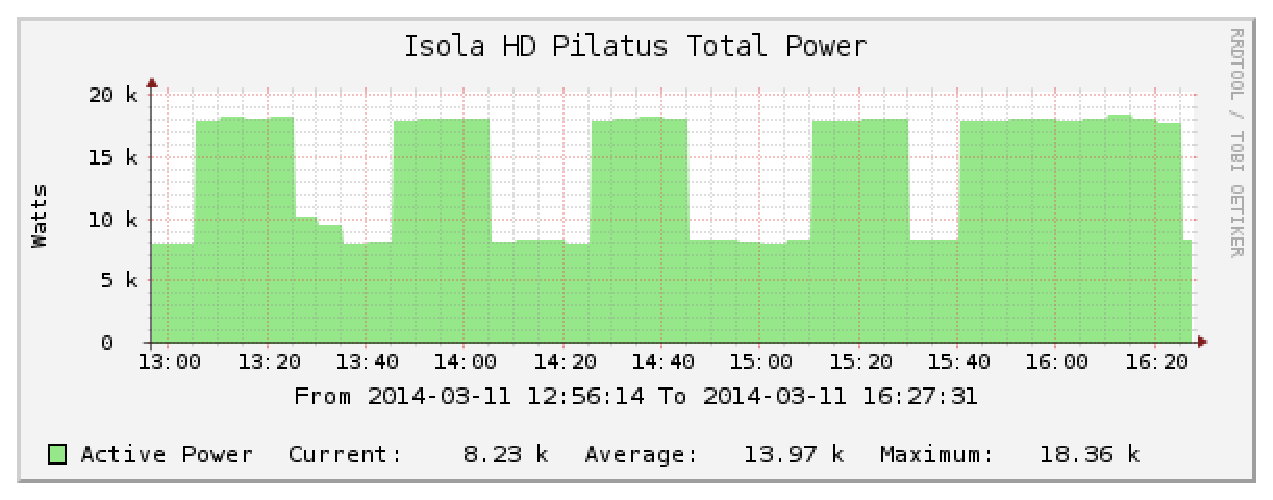
\includegraphics[width=0.48\textwidth]{Figs/NRJ_benchmark_Pilatus.eps}
  \caption{Isola HD total power consumption of \pilat.}
  \label{fig:2}
\end{figure}

\begin{table}[htbf]
  \centering
  \caption{Averaged power consumption (W) of the platforms.}
  \label{tab:1}
  \begin{tabular}{cccc}
    \hline\noalign{\smallskip}     \textbf{\scriptsize{PILATUS}}     &
    \textbf{\scriptsize{MONCH}}  &  \textbf{\scriptsize{TINTORRUM}}  &
    \textbf{\scriptsize{TINTORRUM}}           \\          &          &
    \textbf{\scriptsize{(\emph{Aggressive})}} & \textbf{\scriptsize{(\emph{Degraded})}}
    \\    \noalign{\smallskip}\hline\noalign{\smallskip}   18035.0   &
    12622.5 & 3713.6 & 3651.8 \\ \noalign{\smallskip}\hline
  \end{tabular}
\end{table}

In  Figure~\ref{fig:3}, we  compare both  TTS (right  Y-axis)  and ETS
(left  Y-axis)  metrics  on  both  platforms.  As  expected, Intel Sandy Bridge EP processors of \pilat
outperform the Intel Ivy  Bridge EP processors of \monch, being roughly 130\,\%  faster.  The reason
for that is two-fold: \emph{i}) they have higher clock frequency than Ivy
Bridge  (2.6\,GHz  against  2.2\,GHz),   and  \emph{ii})  they  aim  at
computing   speed  regardless   to  be   energy  efficient.    In  our
experiments,  \monch  showed  the  best  energy-to-solution,
reducing the energy consumption of \pilat by approximately 7\,\%.

Averaged TTS and ETS results  over 10 repetitions of 24h simulation on
\tinto are shown in  Figure~\ref{fig:4}. The corresponding results for
the  averaged total  power are  also shown  in  Table~\ref{tab:1}.  As
expected, the average total power consumption by \cosmoart while using
the \emph{degraded} MPI policy is about  2\,\% less than that consumed by the
\emph{aggressive} one. This is  due to  the reduction of CPU usage (of about 50\,\%) while using  the \emph{degraded} MPI policy, in
contrast with the \emph{aggressive} policy that always yields to 100\,\% of CPU utilization while waiting for an incoming message. From the point of  view of the execution time, there is a
slight reduction  for the \emph{degraded} MPI  policy. One can  expect that the
costs of the context switches produced in the \emph{degraded} MPI policy can lead to
an  increase  of  the   execution  time,  however,  applications  with
extensive computing,  as e.g.  \cosmoart, may show  better performance
with the \emph{degraded} policy. This effect works in  favor with our results
since the energy consumed is also reduced (2\,\%) just by changing the
behavior of the OpenMPI library  to the \emph{degraded} policy, i.e, with the
\texttt{--mca    mpi\_yield\_when\_idle 1}   parameter   set    in   the
\texttt{mpirun} command.

\begin{figure}[htbf]
  \centering
  \includegraphics[width=0.5\textwidth]{Figs/Time_E2S_COSMO-ART-0.eps}
  \caption{Time-to-solution and  energy-to-solution comparison between
    \pilat and \monch for a 24h simulation.}
  \label{fig:3}
\end{figure}

\begin{figure}[htbf]
  \centering
  \includegraphics[width=0.5\textwidth]{Figs/Time_E2S_COSMO-ART-1.eps}
  \vspace{-1cm}
  \caption{Mean time-to-solution and  energy-to-solution on \tinto for
    a 24h simulation using the  \emph{aggressive} and \emph{degraded} MPI policies. The
    95\,\%  confidence  intervals of  Student's  $t$ distribution  (10
    samples) clearly  indicates an improvement for the \emph{degraded} policy in
    both TTS and ETS.}
  \label{fig:4}
\end{figure}

\begin{figure*}[ht]
  \centering
  \hspace{0.8cm} \scalebox{0.62}{\input{Figs/24hour.pstex_t}}
  \caption{24  hours  simulation power  trace  using  the \emph{aggressive}  and
    \emph{degraded} MPI policies on \tinto.}
  \label{fig:5}
\end{figure*}

\begin{figure*}[ht]
  \centering
  \scriptsize
  1 hour simulation during midday (11h--12h) using the \emph{aggressive} MPI policy \\
  \scalebox{0.5}{\input{Figs/11_12_blq0_figure.pstex_t}} \\
  1 hour simulation during midday (11h--12h) using the \emph{degraded} MPI policy \\
  \scalebox{0.5}{\input{Figs/11_12_blq1_figure.pstex_t}} \\
  1 hour simulation during midnight (23h--24h) using the \emph{aggressive} MPI policy \\
  \scalebox{0.5}{\input{Figs/23_24_blq0_figure.pstex_t}} \\
  1 hour simulation during midnight (23h--24h) using the \emph{degraded} MPI policy \\
  \scalebox{0.5}{\input{Figs/23_24_blq1_figure.pstex_t}} \\
  \begin{tabular}{rlp{-0.2cm}rlp{-0.2cm}rlp{-0.2cm}rlp{-0.2cm}rl}
    & &  & &  & &  \\[-0.15cm]
    Computation     & \multicolumn{1}{>{\columncolor[RGB]{  0,  , 255}}p{0.4cm}}{} & & 
    Block. send     & \multicolumn{1}{>{\columncolor[RGB]{255,  0,174}}p{0.4cm}}{} & & 
    Synchronization & \multicolumn{1}{>{\columncolor[RGB]{179,  0,  0}}p{0.4cm}}{} & & 
    Wait/Wait all   & \multicolumn{1}{>{\columncolor[RGB]{235,255,  0}}p{0.4cm}}{} \\
    & &  & &  & &  \\[-0.15cm]
    Immediate recv. & \multicolumn{1}{>{\columncolor[RGB]{100,100,177}}p{0.4cm}}{} & &
    Waiting a msg.  & \multicolumn{1}{>{\columncolor[RGB]{255,  0  ,0}}p{0.4cm}}{} & & 
    Group comm.     & \multicolumn{1}{>{\columncolor[RGB]{255,144, 26}}p{0.4cm}}{} & &
    Others          & \multicolumn{1}{>{\columncolor[RGB]{192,224,  0}}p{0.4cm}}{} \\
    %I/O             & \multicolumn{1}{>{\columncolor[RGB]{172,174, 41}}p{0.4cm}}{} & &
    %
    %Idle            & \multicolumn{1}{>{\columncolor[RGB]{117,195,255}}p{0.4cm}}{} \\
  \end{tabular}
  \caption{Power-performance   traces  during   midday   and  midnight
    leveraging the \emph{aggressive} and \emph{degraded} MPI policies on \tinto.}
  \label{fig:6}
\end{figure*}

\subsection{Power-performance profiling and tracing}
\label{subsec:4.3}

A full tracing  experiment is conducted on \tinto  in order to capture
an overall power profile at a much finer resolution using the attached
PDUs in each  node. First we run \cosmoart for  a 1-day simulation and
analyze the  power consumption.  Second we  correlate performance with
power  traces  of  two  1-hour  time frames  during  the  day:  midday
(11h--12h) and midnight (23h--24h). All the experiments on \tinto were performed
using 192 cores with 12 MPI processes per node, i.e., using an exactly-subscribed MPI mode.

In order to obtain an initial overview of the power consumption of the
system  model,  we  obtained  power  profiles  leveraging  our  \pmlib
power-measurement    framework   over    a    1-day   simulation    of
\cosmoart. These profiles, produced with both \emph{aggressive} and \emph{degraded} MPI
policies,  are depicted in  Figure~\ref{fig:5}. The  first observation
for the \emph{aggressive} MPI policy is that the first and last hours of the day
consume slightly less  power than the midday hours.  We relate these
variations  due   to  the  different   chemical  reactions,  aerosols,
radiations  and clouds  formation processes,  computed by  ART, taking
place during  daylight hours  but not during  night. In this  case the
peak power consumption is about  3821\,W. Looking at the power profile
using the \emph{degraded}  MPI policy, we observe that  the 1-hour pattern is
repeated along  the 24-hours, favoring  the reduction of  power during
night  hours in  a  more noticeable  way  than that  with the   \emph{aggressive}
policy.   The peak  power consumption  during day  hours  while the
 \emph{degraded}  MPI policy  is leveraged  is  about 3768\,W,  which means  a
reduction of around  50\,W with respect to the  \emph{aggressive} mode. Also, we
notice systematic  power drops for each simulated  hour.  We associate
them  to periods  in  which  the processes  were waiting  for
incoming messages  or synchronizations, thus  yielding the CPU  to a lower
usage. Our final observation is the reduction of the TTS by 2\,\% with
respect to the  \emph{degraded} MPI policy.

To  gain  more  insights   about  the  power-performance  behavior  of
\cosmoart,  we  obtained power-per\-for\-man\-ce  traces  to allow  us
correlate  the type  of  tasks  being executed  with  the total  power
consumption  along  the   time  (see  Figure~\ref{fig:6}).   For  this
experiment we  limit the simulation  time to 1 hour  because: \emph{i})
the  pattern of  the computation  performed by  \cosmoart  is repeated
hourly and, \emph{ii}) the weight  of a 1-day simulation trace can not
be easily handled using our  machines and memory available (each trace
file was about 45\,GB). Thus, we shrink the simulations
to 1 hour during midday (from 11h  to 12h) and during
midnight  (from 23h  to  24h), in  which  \cosmoart perform  different
internal computations.  At  the same time we leverage  the two already
stated MPI policies: \emph{aggressive} and \emph{degraded}.

All  the  traces  in   Figure~\ref{fig:6}  are  divided  in  different
computation  phases. In first  phase all  the processes  perform group
communications      and       execute      MPI-receive      primitives
(e.g. \texttt{MPI\_Recv}). The second one performs computation bursts,
combined  in  between   with  group  communications,  blocking  sends,
immediate  receives and  MPI-wait primitives.  Finally,
group  communications interlaced  with computation  and  a significant
synchronization  phase are  performed. From  the performance  point of
view, one can notice a reduction of 2\,\% in the TTS that \emph{degraded}  MPI
mode leads over the \emph{aggressive} MPI  policy. On the other hand an averaged
reduction of power consumption of  2\,\% is attained with the \emph{degraded} 
MPI policy  only in  routines that actually  perform synchronizations,
group  communications  and  MPI-receive/-wait primitives.   Thus,  the
reduction of the power-energy  pair directly depends on the percentage
of time in which blocking MPI  operations are executed. For the 1 hour
simulation traces, an average of 50\,\% of the time the processes were
waiting for incoming messages.  Taking  into account that  the total power  reduction during
blocking phases  is about 5\,\%,  one can compute an  approximation of
the  power savings,  i.e., $50\,\%  \times  5\,\% =  2.5\%$, which  is
consistent  power  reduction  obtained  for  the  full-day  simulation
(around  2\,\%). However,  we  expect higher  power/energy savings  if
upcoming versions of OpenMPI support full blocking policies as well as if 
future architectures tend proportional computing~\citep{Barroso-2007}.

% \begin{figure*}[htbf]
%   \centering
%   Simulation of 1 hour during midnight (from 23h to 24h) leveraging the polling MPI policy\\
%   \includegraphics[width=0.78\textwidth]{Figs/23_24_blq0_stat.eps}\\
%   Percentage of time for the 1 hour during midnight (from 23h to 24h) leveraging the polling MPI policy\\
%   \includegraphics[width=0.78\textwidth]{Figs/23_24_blq1_stat.eps}\\
%   \caption{blabla}
%   \label{fig:7}
% \end{figure*}




\section{Conclusion}
\label{concl}
We  have   presented  a  methodology  for   comparing  performance  of
COSMO-ART,  a  regional  weather  forecast  model  augmented  for  the
interactions of  reactive gases and aerosol  particles.  The resulting
benchmarks illustrate  that the  best time-to-solution does  not imply
the best energy-to-solution: an Intel Sandybridge (2.6 GHz) system has
lower  time-to-solution but  higher energy-to-solution  than  an Intel
Ivybridge  (2.2  GHz) system,  although  the  two  metrics are  indeed
strongly  correlated.   A   tool  utilising  Paraver/Extrae  with  new
extensions  for power  consumption  was successfully  applied to  this
non-trivial application.  The  resulting profiles indicate that simple
changes, such as making use of an MPI version based on blocking rather
than polling, can reduce power consumption significantly.

This  reproducible  benchmark provides  a  baseline  for ongoing  work
package within  the EU-funded Exa2Green to  minimise power consumption
of COSMO-ART. Profiling  has given us insight into  the most expensive
code  components,  which are  now  being  altered  to utilise  revised
algorithms.  The  results of these  optimisations will be  reported in
future publications.


%\paragraph{Paragraph headings} Use paragraph headings as needed.

\begin{acknowledgements}
The research  leading to these  results is supported by  the Exa2Green
project  co-financed by  the European  Commission under  7th Framework
Programme Future and Emerging Technologies (FET) Proactive Initiative:
Minimising Energy  Consumption of Computing to the  Limit (MINECC). We
also gratefully acknowledge the High Performance and High Productivity
Computing Initiative  \citep{HP2C} for results that  will be leveraged
in subsequent code refactoring.
\end{acknowledgements}

\DeclareRobustCommand\IPCClongname{ - Intergovernmental Panel on Climate Change}

\bibliographystyle{plainnat}
\bibliography{\jobname}

\end{document}

